\cia\vspace{-2cm}
\section{Proton Fiducial cuts} 
\label{sec:fid_p} 
Protons  as well as electrons present low efficiency regions. 
Their detection and reconstruction close to boundaries or dead 
channels is not well understood. 

The holes and depletions are treated with the same way as it was done for the electrons.
The depletions, presented as curved bands in $\phi$ versus $\theta$ plots, are shown below 
(\F{fig:proton_tph} and \F{fig:traped_fit_result_s5}).
The reason the bands are curved is that these are related to TOF or DC wires which are straight,
thus not covering regions of $\phi = const$ space.
 
Unlike the electron case, the $\phi$ boundaries are asymmetric, as shown in
\F{fig:proton_tph}.
\begin{figure}[h]
 \begin{center}
 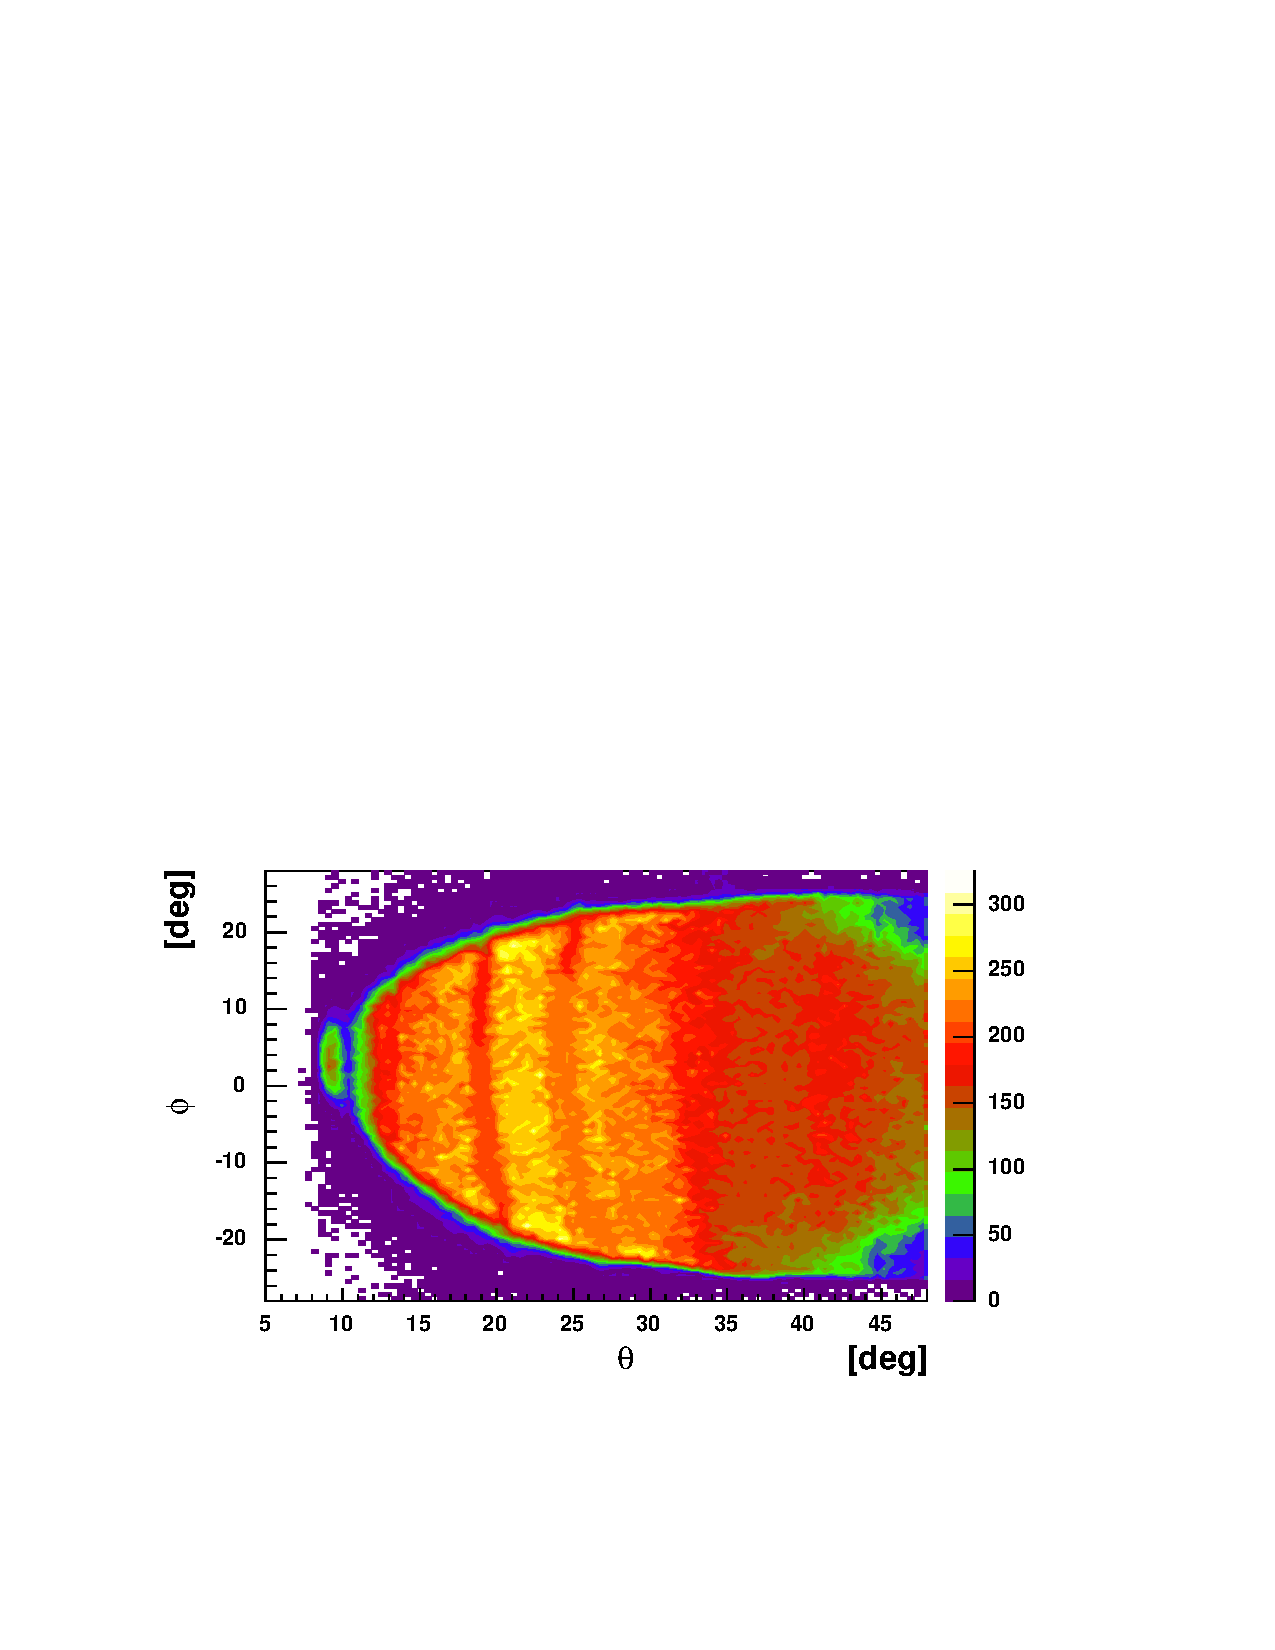
\includegraphics[width = 13cm, bb=40 120 520 420]{data_reduction/img/proton_tph}  
  \caption[$\phi$ versus $\theta$ for sector 5 protons]
           { $\phi$ versus $\theta$ for sector 5. The momentum ranges from $0.9$ 
	              to $1.6$ GeV. The distribution is $\phi$-asymmetric.
                      Depletions along $\phi$ similar to the electron case are visible. }
 \label{fig:proton_tph}
 \end{center}
\end{figure}
\subsection{ $\phi$ boundaries}
In order to evaluate $\phi$ boundaries the momentum has been divided into five bins
equally spaced from $0.9$ to $4.4$ GeV. The momentum 
dependance of the fiducial cut is not as strong as it was for the electrons, so a fewer
number of bins are necessary.

For each momentum bin the $\phi$ distributions were divided in $\theta$ intervals
of $1$ degree and fitted with a trapezoid function \cite{bib:fid_p}. 
The fit gives as output the $\phi$ lower and upper limits in which the $\phi$ distribution
is flat (see \F{fig:traped_fit_s5}). These limits will determine the fiducial cut.

The trapezoid function is shown in \F{fig:traped} and assumes the form
\vspace{0.6cm}
$$
y =\left\{
\begin{array}{c c c c c c c}
  & 0                   &  if & &           &   x \le & p_1-p_0 \\
  & p_4(x-p_1+p_0)/p_0  &  if & & p_1-p_0   & < x \le & p_1\\
  & p_4                 &  if & & p_1       & < x \le & p_2 \\
  & p_4(-x+p_2+p_3)/p_3 &  if & & p_2       & < x \le & p_2 + p_3 \\
  & 0                   &  if & & p_2+p_3   & < x     & 
\end{array}
\right.
$$

\begin{figure}[h]
 \begin{center}
 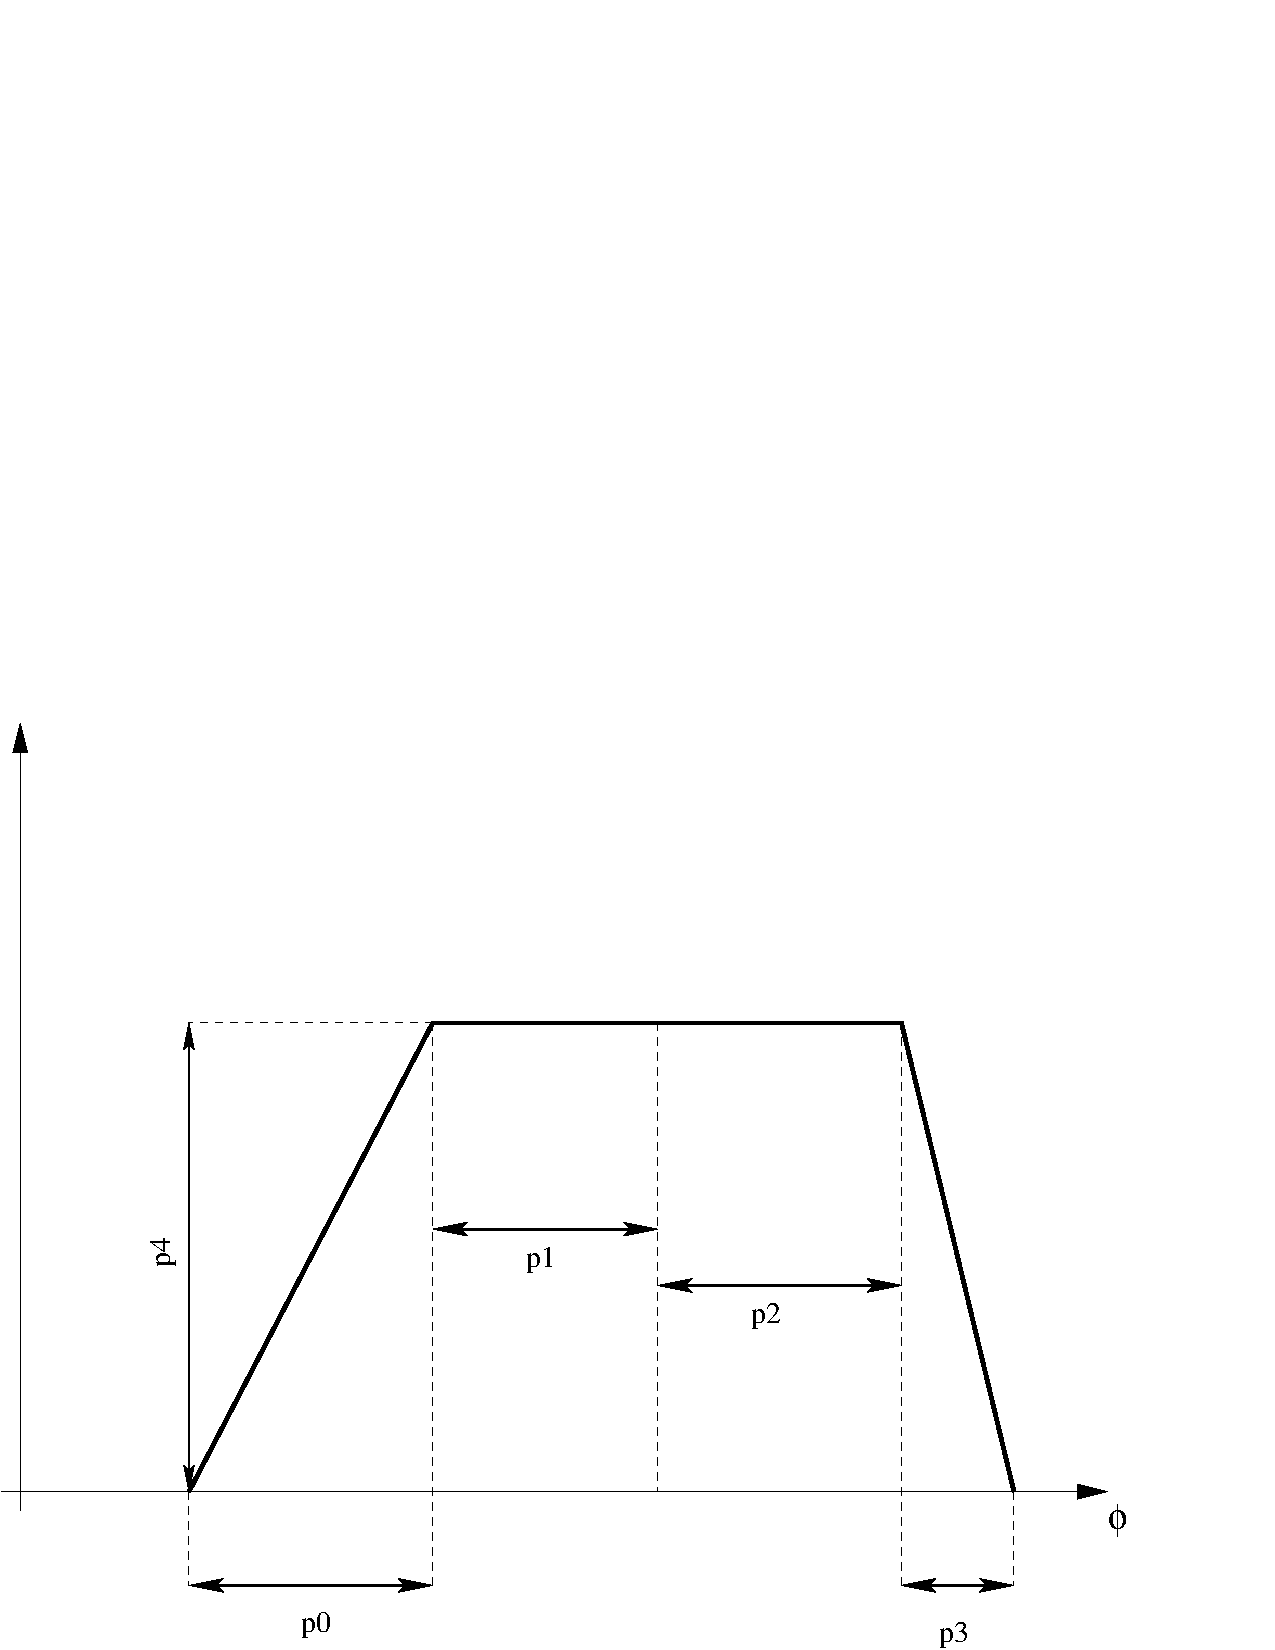
\includegraphics[width = 11cm, bb=-40 20 580 440]{data_reduction/img/traped}  
  \caption[The trapezoid function used for the $\phi$ fit]
          { The trapezoid function used for the $\phi$ fit. The parameters $p_1$ and $p_2$ determine
                     the fiducial cut lower and upper limits.  }
 \label{fig:traped}
 \end{center}
\end{figure}
The trapezoid fit gives the parameters $p_1$ and $p_2$ described above for each $\theta$ considered
in each momentum bin.
These parameters are respectively the $\phi_{MIN}$ and $\phi_{MAX}$ and 
form a $\phi(\theta)$ distribution.


\begin{figure}[tbp]
 \begin{center}
 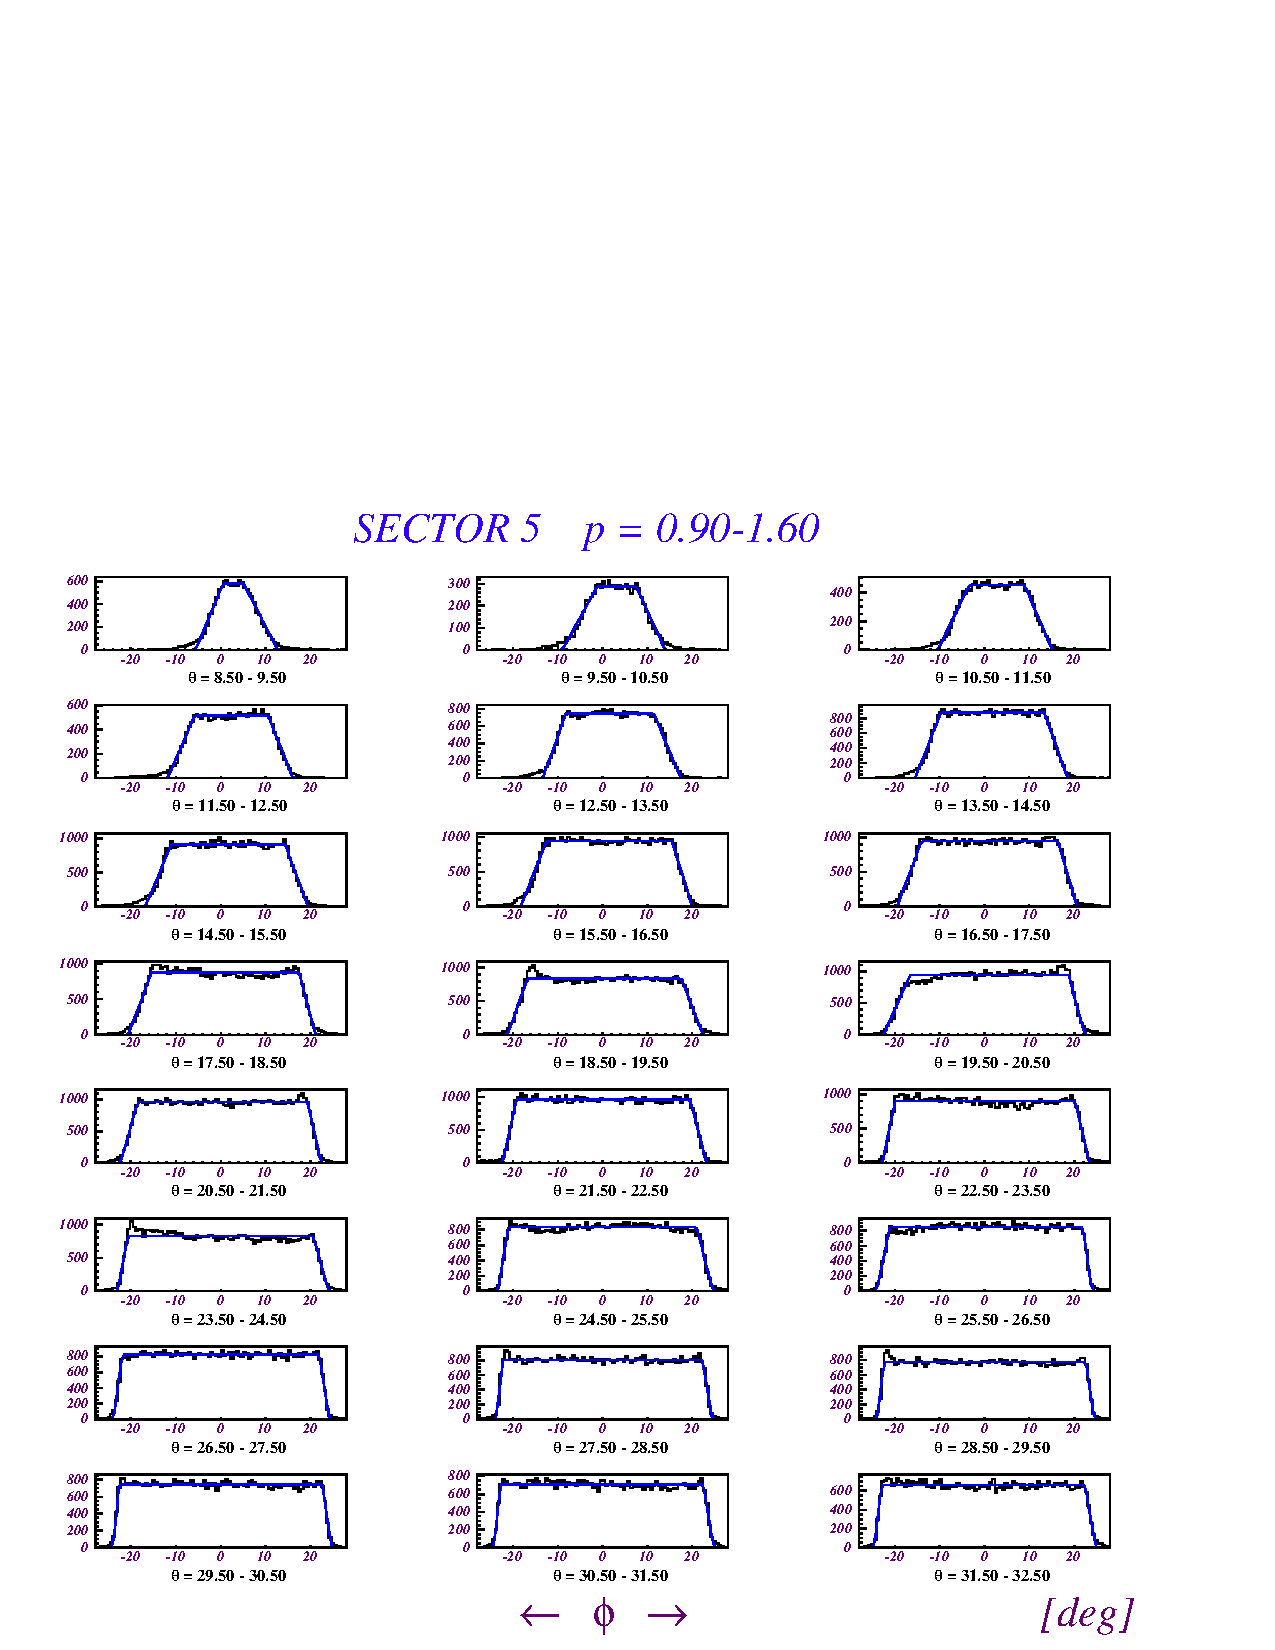
\includegraphics[width = 16cm, bb=0 0 560 560]{data_reduction/img/traped_fit_s5}  
  \caption[Trapezoid fit for sector 5]
          { Trapezoid fit for sector 5. The limits of the flat $\phi$ region of each fit
                     will determine the fiducial cut.}
 \label{fig:traped_fit_s5}
 \end{center}
\end{figure}

\cia


The parameters are fitted as a function 
of $\theta$ with a fourth order polynomial:
$$
\begin{array}{c}
 \phi_{MIN} = a_0 + a_1\theta + a_2\theta^2 + a_3\theta^3 + a_4\theta^4 \\
 \phi_{MAX} = b_0 + b_1\theta + b_2\theta^2 + b_3\theta^3 + b_4\theta^4 \\ 
\end{array}
$$

\F{fig:traped_fit_result_s5} shows the calculated $\phi_{MIN}$ and $\phi_{MAX}$  and the resulting fit 
for sector 5 and momentum range $0.9$ to $1.6$ GeV.

\begin{figure}[h]
 \begin{center}
 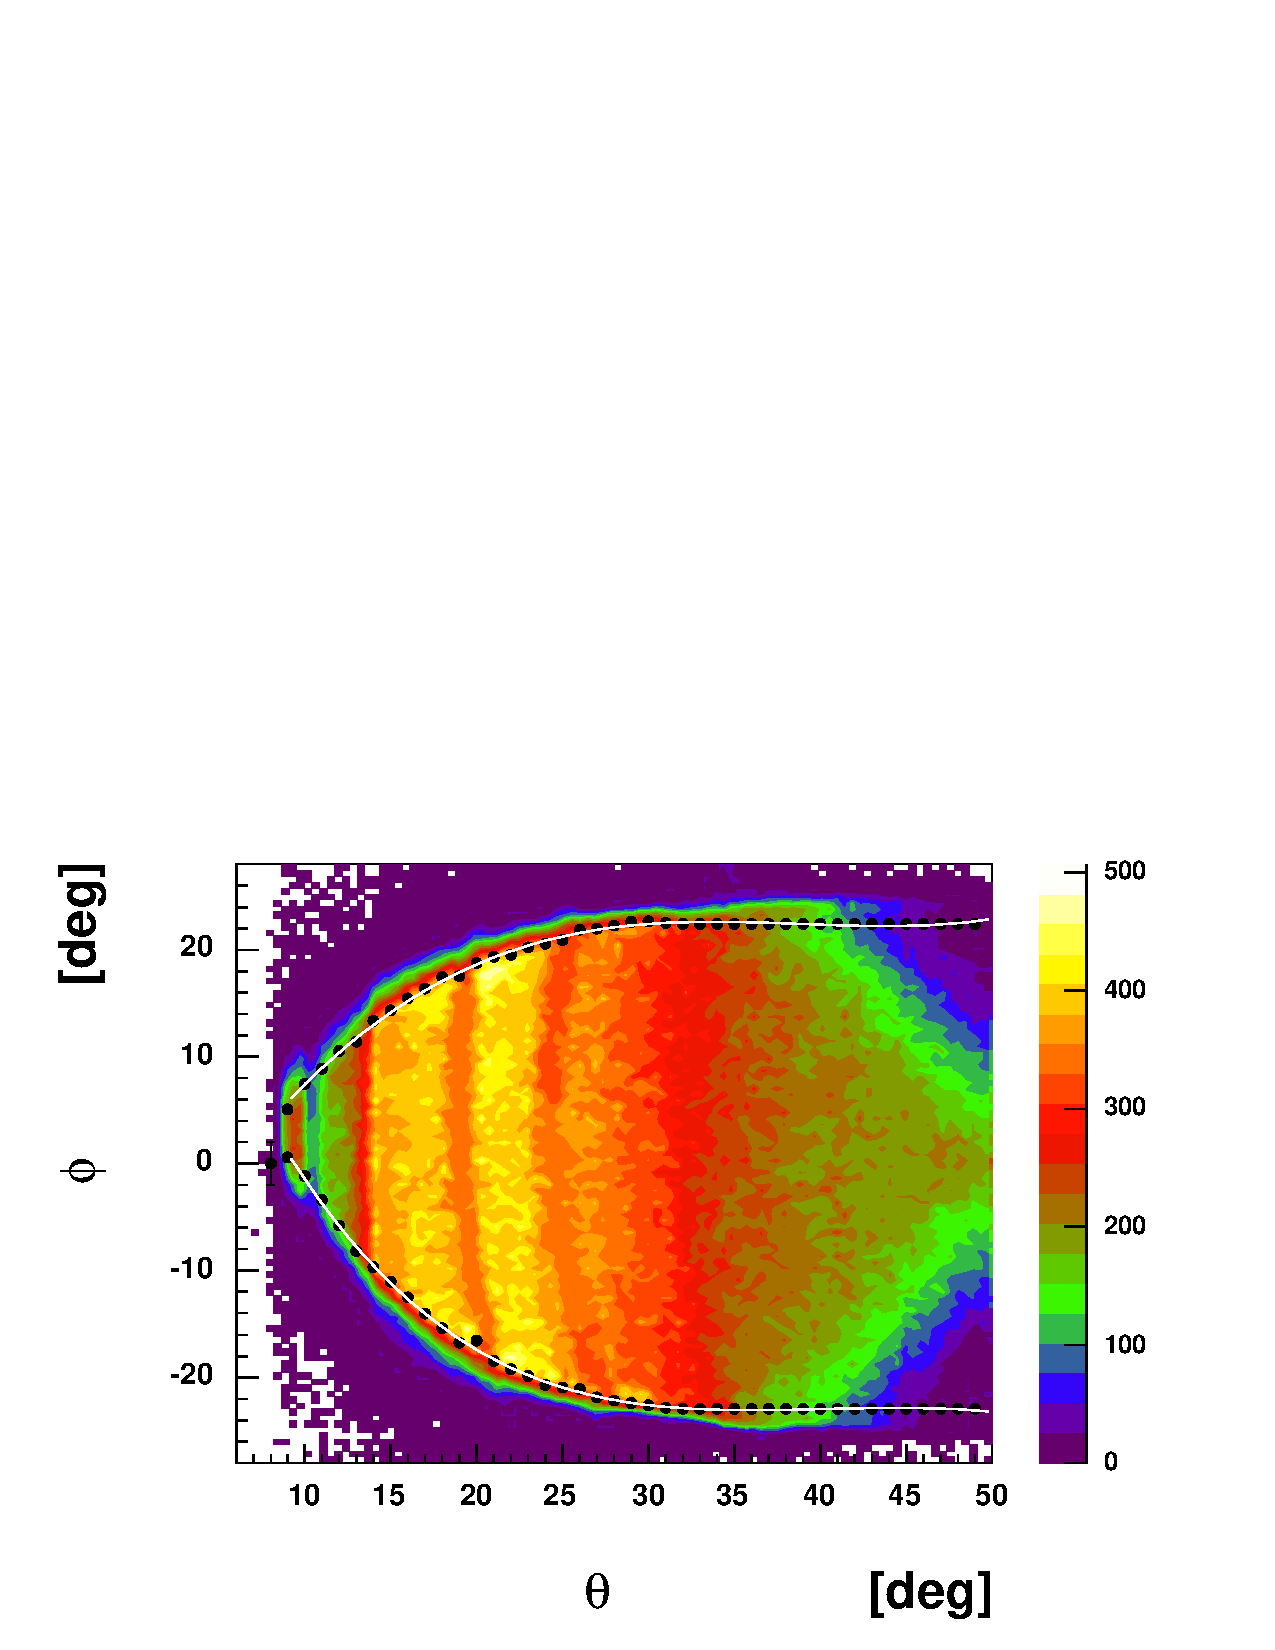
\includegraphics[width = 13cm, bb=0 0 580 430]{data_reduction/img/traped_fit_result_s5}  
  \caption[Result of the trapezoid fit]
          { Result of the trapezoid fit for sector 5. The proton momentum ranges from $0.9$ 
	             to $1.6$ GeV. 
	             The black points are the parameters $p_1$ (negative $\phi$) and $p_2$ (positive $\phi$)
                     for each $\theta$ slice considered as shown in \F{fig:traped_fit_s5}.
		     The white line is a fourth order polynomial fit to the black points.}
 \label{fig:traped_fit_result_s5}
 \end{center}
\end{figure}
\cia
The parameters $a_i , \; b_i $ are momentum dependent, since a fit is made for each momentum bin.
$$
\begin{array}{c}
 a_i = a_i(p) \\
 b_i = b_i(p) \\ 
\end{array}
\,\,\,\,\,i = 0..5
$$
In order to exploit the momentum dependance
each of these parameters is fitted as a function of $p$ 
with a second order polynomial as shown in \F{fig:fid_parameters_fit}.

\begin{figure}[h]
 \begin{center}
 \leavevmode
 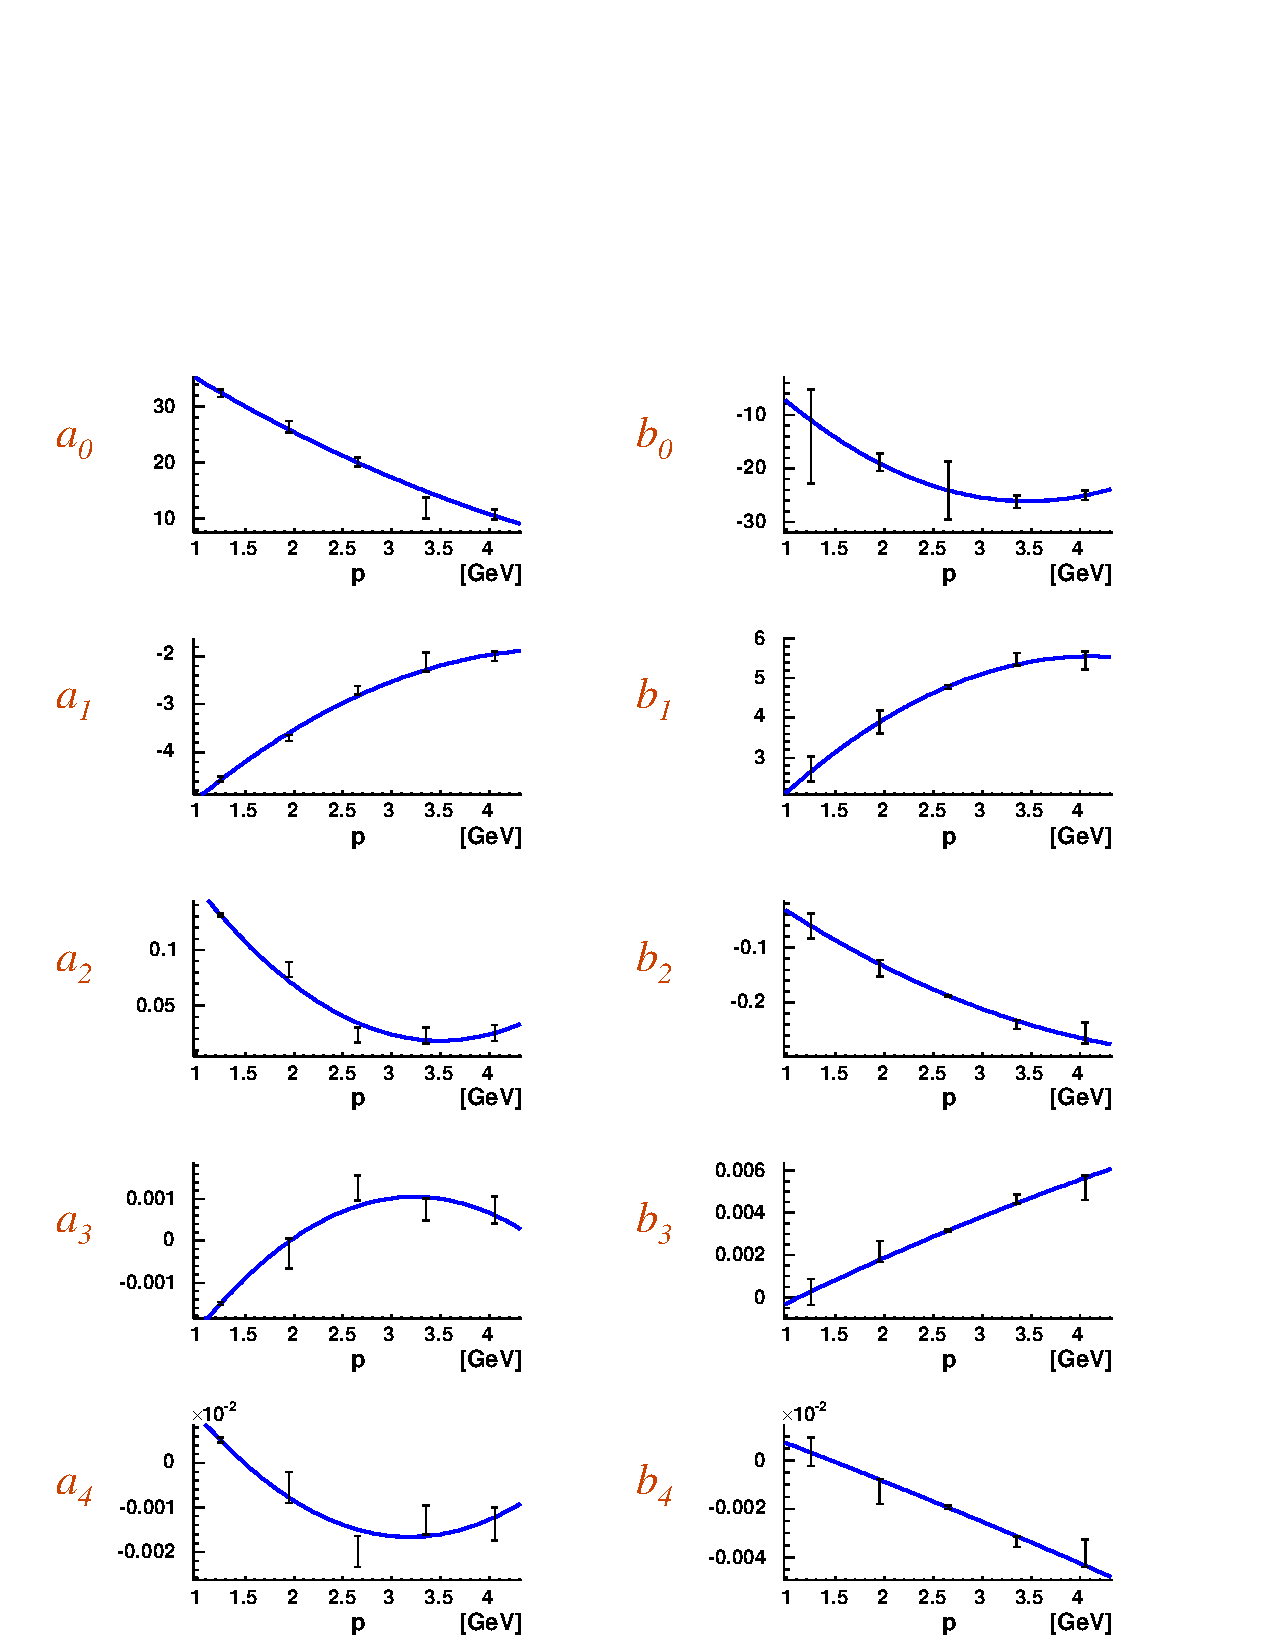
\includegraphics[width = 11cm]{data_reduction/img/fid_parameters_fit}   
  \caption[\boldmath Sector 5 parameters fit]
          { Sector 5 parameters fit. Each of the parameters is fitted as a function
	             of the proton momentum with a second order polynomial.}
 \label{fig:fid_parameters_fit}
 \end{center}
\end{figure}

\cia
The overall fiducial (shown for sector 5 in \F{fig:fid_p_sector5}) cut is finally determined, in each sector, by the limits:
$$
\begin{array}{c}
 \phi_{MIN} = \displaystyle\sum_{i=0}^5 a_i(p)\,\theta^i \\
 \phi_{MAX} = \displaystyle\sum_{i=0}^5 b_i(p)\,\theta^i \\

 \phi_{MIN} \,\le\, \phi \,\le\, \phi_{MAX} \\
\end{array}
$$

\begin{figure}[h]
 \begin{center}
 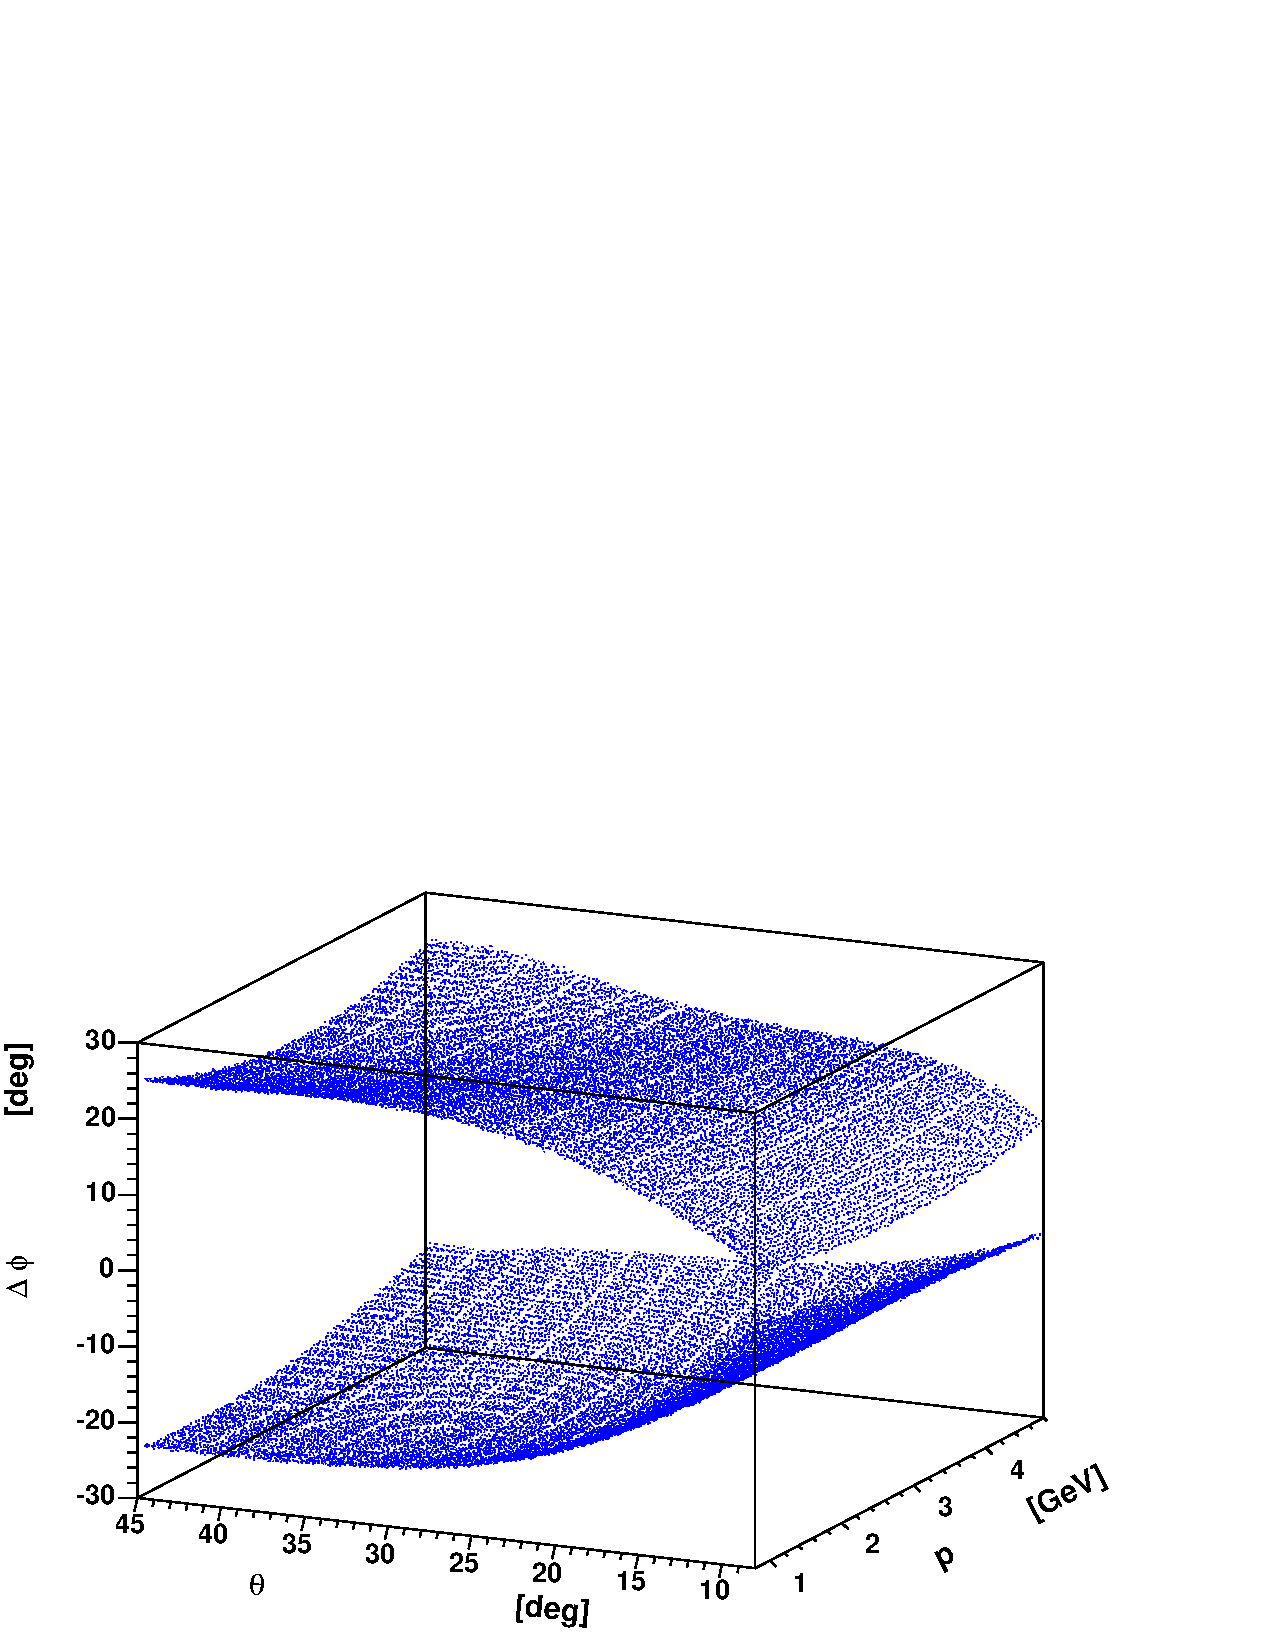
\includegraphics[width = 13cm, bb=0 0 540 380]{data_reduction/img/fid_p_sector5}   
  \caption[Sector 5 $\Delta\phi$ fiducial cut as a function of $\theta$ and $\phi$]
          { Sector 5 $\Delta\phi$ fiducial cut as a function of $\theta$ and $\phi$.}
 \label{fig:fid_p_sector5}
 \end{center}
\end{figure}

\cia

\subsection{ $\theta$ versus momentum cuts}
Sector 2, 3, 5 and 6 present holes and depletions which are taken care of with the 
cuts shown on \F{fig:proton_tp} where $\theta$ is plotted against the momentum $p$.

\begin{figure}[h]
 \begin{center}
 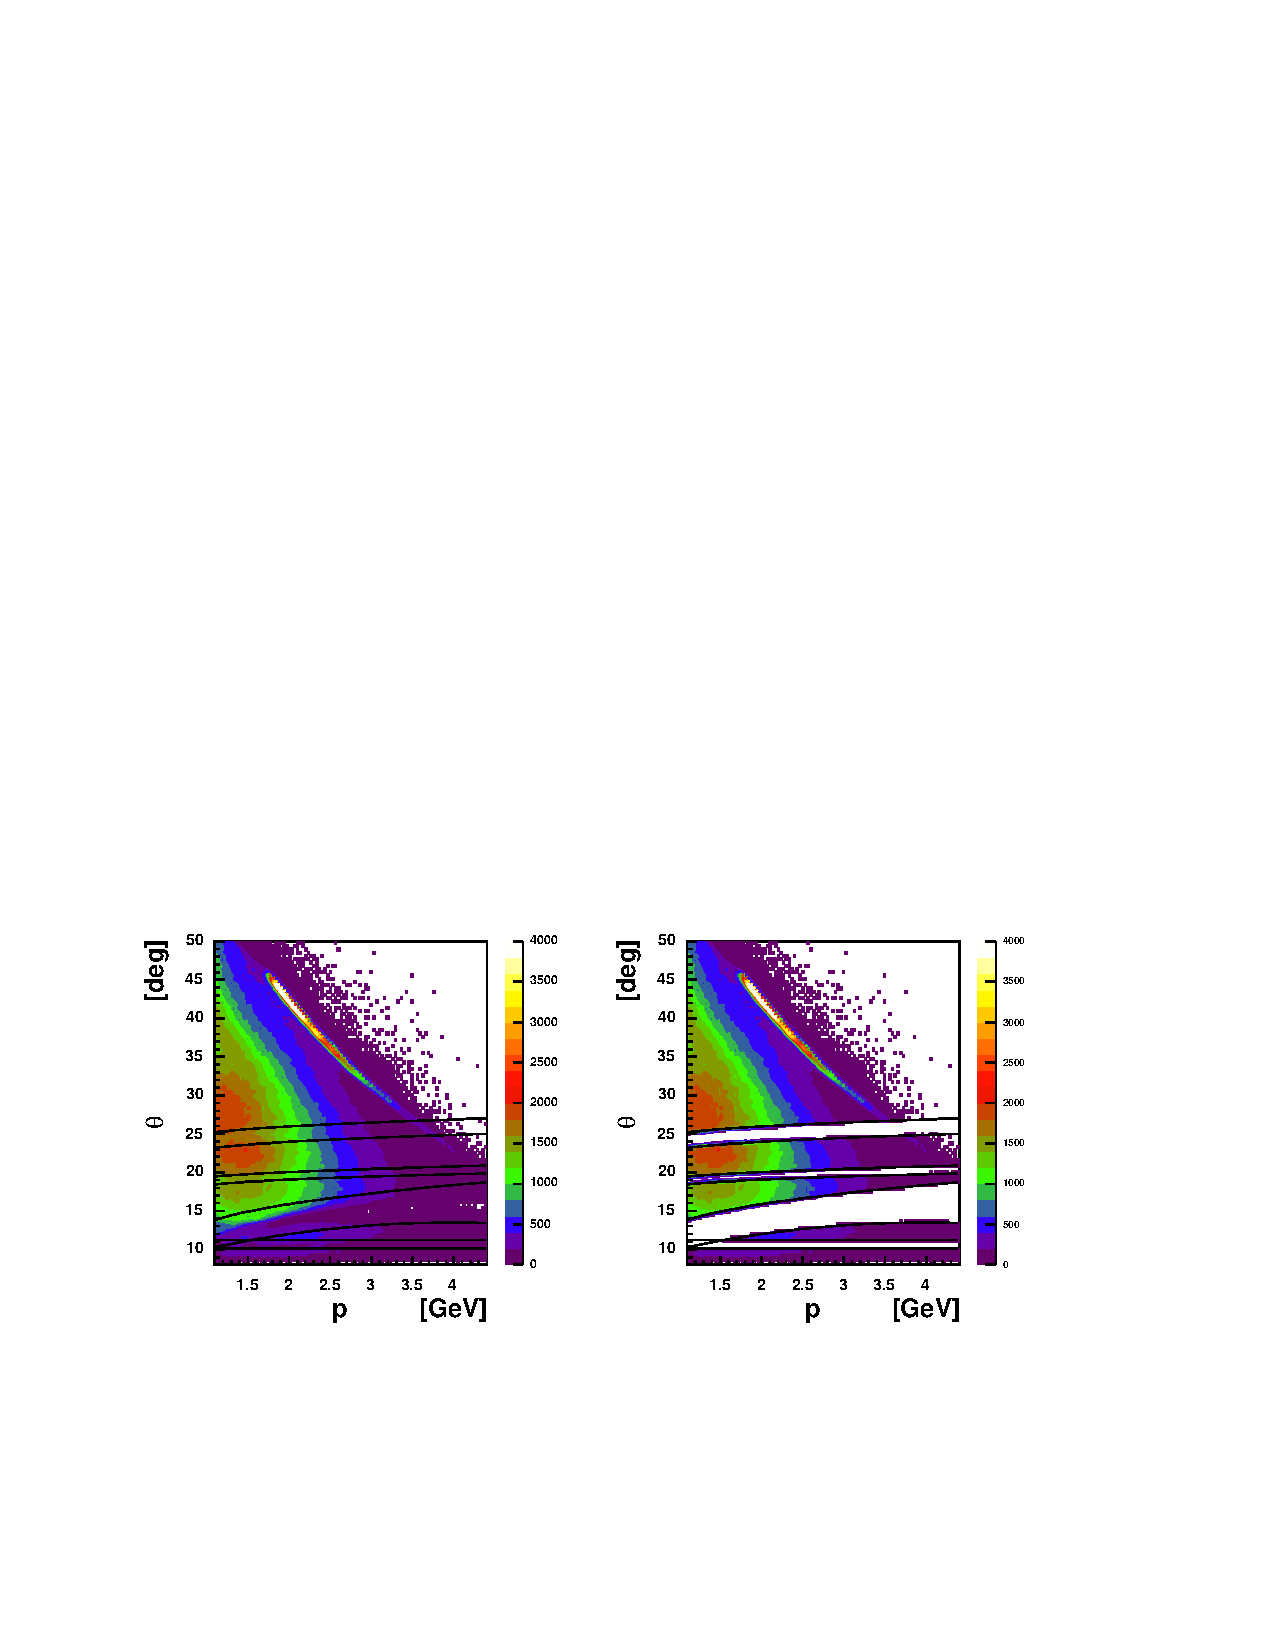
\includegraphics[width = 15cm, bb=20 140 520 380]{data_reduction/img/proton_tp}  
  \caption[$\theta$ versus $p$ for protons sector 5]
          { $\theta$ versus $p$ for protons sector 5. A depletion is clearly visible and cut out.}
 \label{fig:proton_tp}
 \end{center}
\end{figure}

A summary of all parameters can be found in Appendix \ref{app:fidu_p}.

The effect of the fiducial cut on sector 5 is shown in \F{fig:fid_p_sector5_result}.

\cia
\begin{figure}[h]
 \begin{center}
 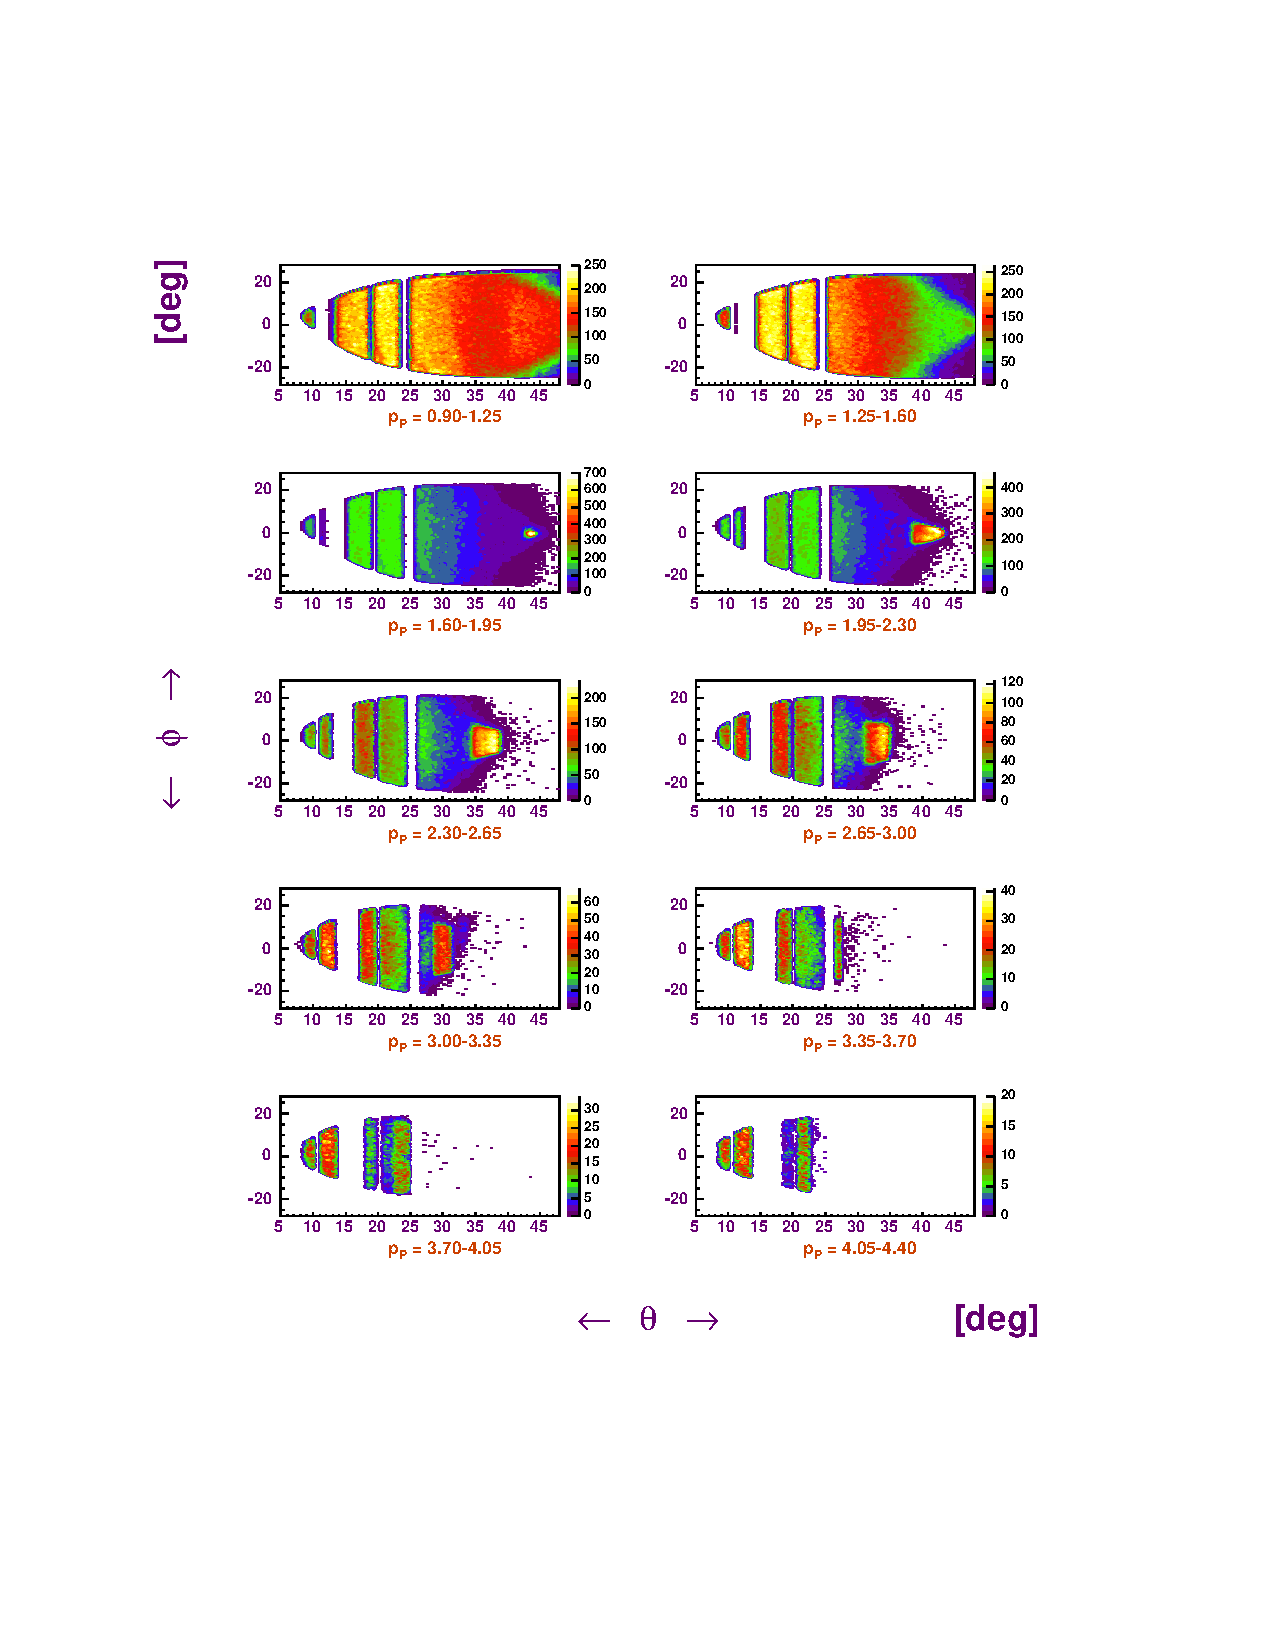
\includegraphics[width = 14cm, bb=60 140 500 660]{data_reduction/img/fid_p_sector5_result}   
  \caption[Sector 5 $\phi$ versus $\theta$ after fiducial cut]
          { Sector 5 $\phi$ versus $\theta$ after fiducial cut. The empty bands
	             in this sector are unfortunate because the forward ones occur 
		     where many protons of interest to us are expected.
		     Compare with \F{fig:proton_tph} or \F{fig:traped_fit_result_s5}
		     to appreciate the cutoff of the depletions.   }
 \label{fig:fid_p_sector5_result}
 \end{center}
\end{figure}














